% Chapter Template

\chapter{Representación de ambiente de ejecución} % Main chapter title
%\section{Reproducibility in scientific workflows using Docker Containers} \label{s4}

%In this paper, we argue that the description of computational environments is necessary for the reproduction of the experiment. Furthermore, the information must be enough to compare and detect differences between the original and the reproduced environments.

En este trabajo, nosotros argumentamos que las descripciones de los ambientes computacionales es necesaria para la reproducción  del experimento. Además, la información debe ser la suficiente para comparar y detectar las diferencias entre el ambiente original y el reproducido.

Dada que las imágenes Docker son un ambiente aislada y independiente, los componentes de software dentro del container están relacionado al experimento y no existen componentes no relacionados. 
Por esta razón, nosotros aseguramos que las anotaciones no presentarán ruido de otras herramientas o dependencias asociadas.
Para realizar una anotación automática de los paquetes instalados, nosotros proponemos, e implementamos un sistema de anotación.
El sistema requiere el nombre de una imagen existente en un repositorio de DockerHub y opcionalmente los datos del repositorio Git que almacena el archivo Dockerfile. 

Los pasos asociados del sistema anotación:

\begin{enumerate}
	\item Consultar a repositorio los metadatos de la imagen. Anotar los metadatos utilizando la ontología propuesta.
	\item Descargar cada una de las capas asociadas a la imagen Docker.
	\item Utilizar Clair, Clair monta cada una de capas de la imagen, detecta los componentes de software instalados utilizando el sistema de paquete.
	\item Obtener la información de Clair, anotar los datos obtenidos por Clair según la ontología.
	\item Guardar los datos en una base de datos RDF que permita consulta SPARQL.
\end{enumerate} 

%----------------------------------
% 4.1 Semantic models
%----------------------------------
\section{Semantic models}\label{s4.1}
     
En \cite{santana2017reproducibility}, los autores proponen \emph{The Workflow Infrastructure Conservation Using Semantics ontology (WICUS)}. WICUS es ontología OWL2 (Web Ontology Language) que implementa la conceptualización de los principales dominios de la infraestructura computacional. Estas son: Hardware, Software, Workflow y recursos de computo
     
Los autores definen que los workflows cientificos requieren un conjunto de componentes de software, y los investigadores deben conocer como desplegar estos componentes para lograr ambiente equivalente.
Por lo tanto, nosotros utilizamos algunos clases y relaciones desde la ontología WICUS:

\begin{description}
	\item [DeploymentPlan:]  Un plan de despliegue está compuesto de todos los pasos  
	\item 
	El plan de despliegue permite entender al investigador cuáles fueron los pasos requeridos para construir el ambiente computacional.
	\item [DeploymentStep:] Cada paso de despliegue es representado por una línea de comando que realiza la instalación, descarga o configuración del ambiente. La información se obtiene desde el archivo DockerFile
	\item [ConfigurationInfo:]
	\item [ConfigurationParameter:]  
	\item [SoftwareStack:]
	\item [SoftwareComponent:]
\end{description} 


Definimos \verb|SoftwarePackage| como una subclase de \verb|SoftwareComponent| para definir los componentes instalados por el gestor de paquetes del sistema operativo y \verb|CondaPackage| los componentes instalados por el sistema de paquetes Conda.
Cada \verb|wicus:SoftwareComponent| tiene una relación \verb|dockerpedia:hasVersion| que muestra la versión del software instalado.

\todo[inline]{P4.1.2 Explicación de los cambios en la ontología}

Our final ontology is depicted in Figure~\ref{fig:ontology}. 

\begin{figure}
  \caption{Docker ontology.}
  \centering
    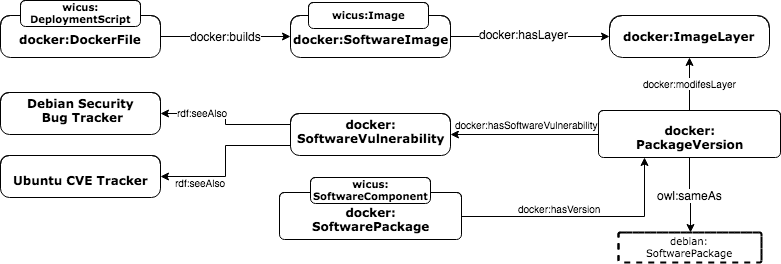
\includegraphics[width=0.4\textwidth]{Figures/dockerOntologyBasic.png}
    \label{fig:ontology}
\end{figure}



%----------------------
% 4.2 Annotator
%-----------------------
\section{Annotator}\label{s4.2}

%url de repositorio github y ubicación del Dockerfile
El servicio de anotación utiliza una interfaz REST para recibir la imagen Docker del experimento científico. Opcionalmente, el usuario puede entregar la información sobre el repositorio Git.  

 El sistema anotación realiza dos tipos de anotaciones: Componentes de software y pasos de construcción 

 
%--------------------------------------------
% 4.2.1 Building steps annotations
%---------------------------------------------
\subsection{Building steps annotations}\label{s4.2.1}

Anotamos el plan de despliegue (Deployment Plan) usando dos métodos. El primero método obtiene los pasos desde el archivo Dockerfile entregado por el usuario, esto permite obtener los pasos y la ubicación de archivo en el repositorio. 

Este método asegura la reconstrucción del ambiente debido a que cualquier archivo necesario por Dockerfile se encuentra en el repositorio Git.

Sin embargo, un usuario puede construir una imagen sin compartir el archivo Dockerfile. ~\cite{}. reporta que el 30\% de las imágenes Docker en DockerHub enlanza su archivo Dockerfile. 

Por lo tanto, nosotros extraemos la información utilizando el manifesto de la imagen Docker. Según la documentación de Docker, el manifiesto de la imagen provee la configuración y el conjunto de las capas de la imagen

Algunos atributos importantes son:

\begin{description}
	\item [name:] \textit{string} name is the name of the image’s repository
	\item [tag:] \textit{tag} is the tag of the image
	\item [architecture:] \textit{string} architecture is the host architecture on which this image is intended to run. This is for information purposes and not currently used by the engine
	\item [fsLayers:] \textit{array} fsLayers is a list of filesystem layer blob sums contained in this image. \\ 
		An fsLayer is a struct consisting of the following fields:
		\begin{description}
			\item [blobSum:] blobSum is the digest of the referenced filesystem image layer. A digest must be a sha256 hash
		\end{description}
	\item [history]: \textit{array} history is a list of unstructured historical data for v1 compatibility. It contains ID of the image layer and ID of the layer’s parent layers. A history is a struct consisting of the following fields:
	\begin{description}
		\item[v1Compatibility]:  \textit{string} V1Compatibility is the raw V1 compatibility information. This will contain the JSON object describing the V1 of this image. A V1Compatibility is a struct consisting of the following fields:
		
		\begin{description}
			\item [Id:] \textit{string} ID of the layer using sha256 hash
			\item [Parent:] \textit{string} ID of the parent layer using sha256 hash
			\item [ContainerConfig:] \textit{string} The command that built the layer
			\item [Author:] \textit{string} The name and email of the author
		\end{description}
	\end{description}
\end{description}

\todo[inline]{P4.3.3 Explicar como guardamos la información en RDF}


\todo[inline]{P4.3.4 Mostrar un ejemplo de anotación}

%--------------------------------------------
% 4.2.2 Software Components annotations
%---------------------------------------------
\subsection{Software Components annotations}\label{s4.2.2}


Nosotros lograr la anotación de los componentes de software utilizando los sistemas de paquetes del sistema, un sistema de paquete es una colección de herramientas de software que automatizan la instalación, actualización, configuración y eliminación de componentes de software. 
Clasificamos los sistemas que paquetes en dos tipos: sistemas de paquetes del sistemas y generales:

\begin{description}
	\item  [Sistemas de paquetes de sistema:] son aquellos vinculados al sistema operativo (e.g., apt de familia Debian, yum de familia RedHat).
	\item [Sistemas de paquetes generales:] son aquellos externos que normalmente son utilizados para instalar un componentes de software de tercero ó un lenguaje especifico (e.g., pip, conda, npm). Conda es un sistema paquete frecuentemente utilizado por investigadores al estar relacionado con Jupyter Notebook.

\end{description}

%We achieve the software components annotations using software package manager, a package manager system is a collection of software tools that automate the process of installing, upgrading, configuring, and removing software components. 

\subsection{Desafios}\label{s4.2.2}

La descripción de los componentes de software es fundamental para realizar cuantificar la similitud entre dos o más ambientes computacionales.
Un enfoque común para detectar los componentes de software guardar o detectar los comandos que realizan la instalación de software. Por ejemplo, la figure \ref{} muestra los comandos para instalar los componentes de la imagen TensorFlow. 


\begin{lstlisting}
apt-get install -y --no-install-recommends \
        build-essential \
        curl \
        libfreetype6-dev \
        libhdf5-serial-dev \
        libpng12-dev \
        libzmq3-dev \
        pkg-config \
        python \
        python-dev \
        rsync \
        software-properties-common \
        unzip	
\end{lstlisting}

El enfoque detectaría los componentes: build-essential, curl, libfreetype6-dev, libhdf5-serial-dev, libpng12-dev, libzmq3-dev, pkg-config, python, python-dev, rsync, software-properties-common y unzip. Sin embargo, el enfoque no obtiene información sobre las versiones o las dependencias del software. Utilizando nuestra propuesta, se puede terminar que el línea anterior instala 184 paquetes.
Para realizar esta tarea, nosotros utilizamos y extendemos Clair. Clair es una herramienta open-source diseñada para identificar vulnerabilidades en imágenes Docker. Clair ha sido utilizada principalmente para analizar imágenes en los repositorios privados de CoreOS, pero puede ser utilizados para analizar distintos repositorios.

Clair descarga todas las capas de una imagen como un sistema de archivo \textit{file system}, analiza los componentes de software instalados en cada capa. 
Finalmente, el resultado del análisis es una lista de los paquetes instalados en la imagen, las capas asociadas con la imagen y sus relaciones.
Clair es compatible con los sistemas de paquetes de las siguientes distribuciones de Linux: Ubuntu, Debian, Alpine, Redhat, CentOS y Oracle. Sin embargo, Clair no es compatible con sistemas de paquetes generales.
Considerando la popularidad de Jupyter Notebook y conda en la comunidad científica, nosotros extendemos Clair para detectar los paquetes instalados por Conda en la imagen.

\todo[inline]{P4.4.5 Mostrar un ejemplo de anotación en RDF}

\begin{lstlisting}
\end{lstlisting}

%-----------------------------------------------
% 4.3 Reproduce and compare the new environment
%-----------------------------------------------
\section{Reproduce and compare the new environment}\label{s4.3}
\todo[inline]{P4.5.1 ¿De que sirve todo esta conservación lógica y porque RDF o SPARQL?}


\todo[inline]{P4.5.2 Ejemplo de como crear una nueva imagen a través de las anotaciones de la conservación lógica}



\todo[inline]{P4.5.3 Ejemplo de dos containers distintos como se que me falta}


\todo[inline] Best practices to ensure reproducibility utilizando docker
